\documentclass[12pt]{article}
\usepackage{enumitem}
\usepackage[letterpaper,left=2cm,right=2cm,top=2cm,bottom=2cm]{geometry}
\usepackage{tikz-cd,amsmath,amssymb}
\usepackage{graphicx}
\newenvironment{QandA}
{
	\begin{enumerate}[label=\normalfont\arabic*.,leftmargin=2em,rightmargin=2em]\normalfont
	}
	{
	\end{enumerate}
}
\newenvironment{codelalala}{}{}
\newenvironment{answered}{\setlength{\parindent}{1em}\par\normalfont}{}
\usepackage{lipsum}
\pagestyle{empty}
\title{CSE 573 Fall 2018 Project 1}
\author{Pratik Pravin Kubal}
\date{UB Person Number: 50290804}
\pagestyle{plain}
\begin{document}
	\noindent%
	\maketitle
	\begin{QandA}
		\item Edge Dectection
		\\
		\\
			Write programs to detect edges in Fig. 1 (along both x and y directions) using Sobel operator. In your report, please include two resulting images, one showing edges along x direction and the other showing edges along y direction.
	\begin{answered}
		For Edge detection firstly I used the basic functions from cv library to read and write. While working on it, previously I had Normalized directly by taking the value 255 as the max value. However, later on I used absolute values method given in "demo.py". Both methods gave similar results.
		\\
		The Normalization used: 
		abs(image)/max(abs(image))
		\\
		Since I am using float array, I had problem writing the image, it was black because the values of pixels were very less, therefore, I multiplied the pixel values by 255 to get an image that I can write.
		\\
		\begin{figure}
		\centering
  			\fbox{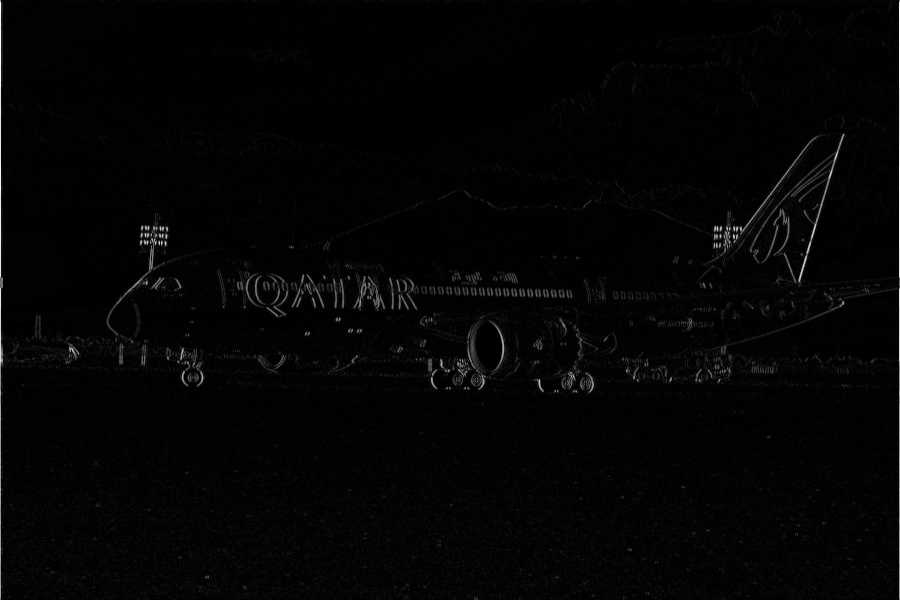
\includegraphics[scale=0.25]{./edge_x.jpg}
  					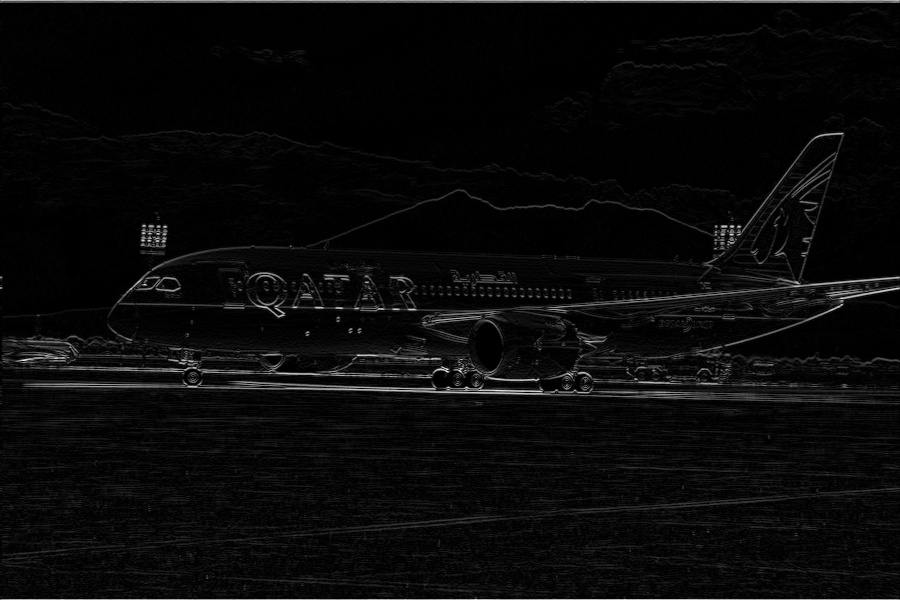
\includegraphics[scale=0.25]{./edge_y.jpg}}
  			\caption{Edge Detection along x axis and y axis }
  		\label{edge-detection}
\end{figure}
		For functions used to build Edge detection are as follows:
		\begin{codelalala}
		\begin{verbatim}
		def rgbToGrayscale(image):
    		r,g,b = image[:,:,0],image[:,:,1],image[:,:,2]
    		grayscaleImage =  0.299*r + 0.587*g + 0.114*b
    		return grayscaleImage
    	\end{verbatim}
		\begin{verbatim}
		def windowMult(matA,matB):
    		matResult = 0
    		for x_iter in range(0,getShape(matA)[0]):
        		for y_iter in range(0,getShape(matA)[0]):
            		if not len(matA) or not len(matB) == 0:
                		matResult += matA[x_iter][y_iter] * matB[x_iter][y_iter]
    		return matResult
		\end{verbatim}
		\begin{verbatim}
		def padMat(matA,sizeWindow):
    		space = (int)(sizeWindow/2)
    		skeleton=[[] for i in range(0,(getShape(matA)[0]+(space*2)))]
    		for window_h in range(0,getShape(matA)[0]+(space*2)):
        		for window_w in range(0,getShape(matA)[1]+(space*2)):
            		if(window_h >= 0 and window_h <= (space-1)) or 
            		(window_h >getShape(matA)[0]+(space-1) 
            		and window_h <= getShape(matA)[0]+((space*2)-1) ):
                		skeleton[window_h].append(0)
            		else:
                		if(window_w >= 0 and window_w <= (space-1)) or 
                		(window_w > getShape(matA)[1]+(space-1)
                	 	and window_w <= getShape(matA)[1]+((space*2)-1)):
                    		skeleton[window_h].append(0)
               			else:
                    		skeleton[window_h].append(matA[window_h-(3)][window_w-(3)])
    		return skeleton
		\end{verbatim}
		\begin{verbatim}
		def sliceMat(matrix,window_h_start,window_h_stop,window_w_start,window_w_stop):
    		retMat = matrix[window_h_start:window_h_stop]
    		holdWindow = []
    		for i in range(0,len(retMat)):
        		holdWindow.append(retMat[i][window_w_start:window_w_stop])
    		return holdWindow
		\end{verbatim}
		\begin{verbatim}
		def normImage(matA):
    		skeleton=[[] for i in range(0,getShape(matA)[0])]
    		maxValue = 0
    		absValue = 0
		    for window_h in range(0,getShape(matA)[0]):
		        for window_w in range(0,getShape(matA)[1]):
        		    absValue = abs(matA[window_h][window_w])
		            skeleton[window_h].append(absValue)     
        		    if(maxValue < absValue) : 
        		    	maxValue = absValue
			returnMat=[[] for i in range(0,getShape(matA)[0])]
		    for window_h in range(0,getShape(matA)[0]):
        		for window_w in range(0,getShape(matA)[1]):
            		returnMat[window_h].append(skeleton[window_h][window_w] / maxValue)
    		return returnMat
		\end{verbatim}
		\begin{verbatim}
		def getShape(matA):
    		height = len(matA)
    		width = len(matA[1])
    		for i in range(0,height):
        		if(len(matA[i]) != width):
            		return -i
        		else:
            		return (height,width)
		\end{verbatim}	
    	\begin{verbatim}
		def invertMat(matA):
    		skeleton=[[] for i in range(0,getShape(matA)[0])]
    		i = 0
    		for window_h in range(getShape(matA)[0]-1,-1,-1):
        		for window_w in range(getShape(matA)[1]-1,-1,-1):
            		skeleton[i].append(matA[window_h][window_w])
       			i += 1
    		return skeleton
		\end{verbatim}
		\begin{verbatim}
def combineEdges(matA,matB):
    from math import sqrt
    maxValue = 0
    skeleton = [[] for i in range(0,getShape(matA)[0])]
    for window_h in range(0,getShape(matA)[0]):
        for window_w in range(0,getShape(matA)[1]):
            skeleton[window_h].append(sqrt(matA[window_h][window_w]**2 + matB[window_h][window_w]**2))
    for window_h in range(0,getShape(skeleton)[0]):
        for window_w in range(0,getShape(skeleton)[1]):
            if(skeleton[window_h][window_w]>maxValue): maxValue = skeleton[window_h][window_w]
    for window_h in range(0,getShape(skeleton)[0]):
        for window_w in range(0,getShape(skeleton)[1]):
            skeleton[window_h][window_w] = skeleton[window_h][window_w]/maxValue
    return skeleton
\end{verbatim}
		For actual sobel operator convolution I have used the following functions:
		\begin{verbatim}
		def sobel(matA,sobel_op):
    		matA = padMat(matA,3)
    		resultImage = [[]for i in range(600)]
    		for window_h in range(0,getShape(matA)[0]-2):
        		for window_w in range(0,getShape(matA)[1]-2):
            		window = sliceMat(matA,window_h,window_h+3,window_w,window_w+3)
            		opResult = windowMult(sobel_op,window)
            		resultImage[window_h].append(opResult)
    		resultImage = normImage(resultImage)
    		return resultImage
		\end{verbatim}
		The whole code which depends on these above functions is:
		\begin{verbatim}
from functions import rgbToGrayscale,windowMult,padMat,sliceMat,
normImage,getShape,invertMat,combineEdges,sobel
import numpy as np
import cv2

# Reading the Image
a = cv2.imread("./proj1_cse573/task1.png")
b = rgbToGrayscale(a)

# Define Operators
sobel_op_x = [[1,0,-1],
              [2,0,-2],
              [1,0,-1]]
sobel_op_y = [[-1,-2,-1],
              [0,0,0],
              [1,2,1]]

# Sobel Edges in x
edge_x = sobel(b,invertMat(sobel_op_x))

# Converting the image to display and write using cv libraries
edge_x_norm = np.asarray(edge_x)
edge_x_norm = edge_x_norm * 255
edge_x_norm = edge_x_norm.astype('uint8')
cv2.imwrite("edge_x.jpg",edge_x_norm)

# Sobel Edges in x
edge_y = sobel(b,invertMat(sobel_op_y))


# Converting the image to display and write using cv libraries
edge_y_norm = np.asarray(edge_y)
edge_y_norm = edge_y_norm * 255
edge_y_norm = edge_y_norm.astype('uint8')
cv2.imwrite("edge_y.jpg",edge_y_norm)

# Combining edge detection in x and y
combined = combineEdges(edge_x,edge_y)
combined_norm = np.asarray(combined)
combined_norm = combined_norm * 255
combined_norm = combined_norm.astype('uint8')
cv2.imwrite("combined.jpg",combined_norm)

print("Original image size: {:4d} x {:4d}".format(a.shape[0], a.shape[1]))
print("Resulting image size: {:4d} x {:4d}".format(combined_norm.shape[0], combined_norm.shape[1]))
		\end{verbatim}
		\end{codelalala}
		Observations:
		\\
		Edge detection along x and y directions have been computed(See Fig \ref{edge-detection}). I have also combined both the edges,see Fig. \ref{edge-detection-combined}. When I was using the old basic divide by 255 normalization, I was missing few edges however, when I used the absolute valued normalization, the results were better.
	\begin{figure}
		\centering
  			\fbox{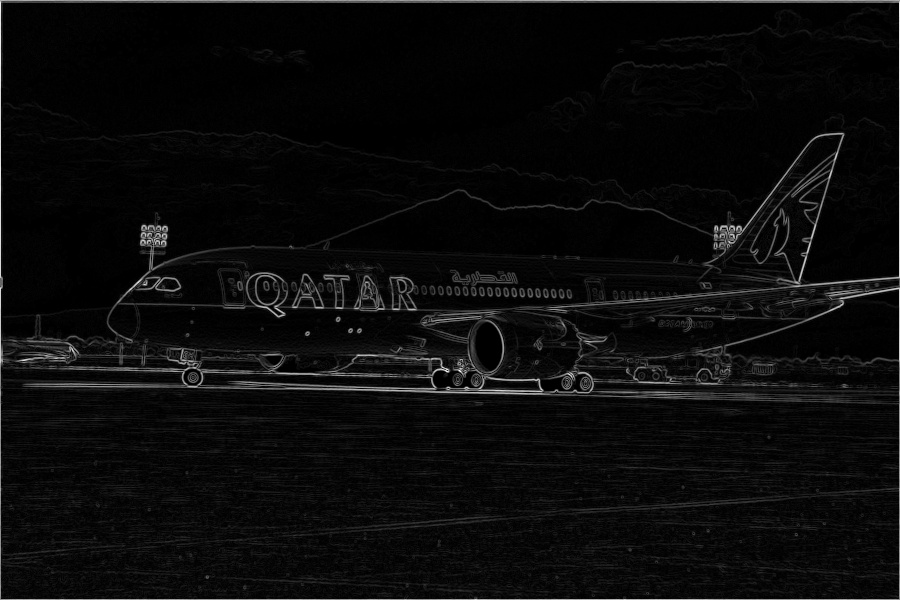
\includegraphics[scale=0.25]{./combined.jpg}}
  			\caption{Combined edge detected in x and y axis}
  		\label{edge-detection-combined}
	\end{figure}
	\end{answered}
	\item Keypoint Detection
	\\
	\\
	Write programs to detect keypoints in an image according to the following steps, which are also the first three steps of Scale-Invariant Feature Transform (SIFT).
\\
1.	Generate four octaves. Each octave is composed of five images blurred using Gaussian kernels. For each
octave, the bandwidth parameters σ (five different scales) of the Gaussian kernels are shown in Tab. 1.
\begin{answered}
I am using the method discussed by the TA and used by openCV of multiplying with the constant to generate Gaussian Kernel. The formula for it is as follows:
\\
C = $\frac{1}{\sum_{i=-2}^{2}\sum_{j=-2}^{2}f(i,j)}$
\\
Where, f(i,j) is the gaussian function
\\
The functions used for this task is as follows:
\begin{codelalala}
\begin{verbatim}
def genOctave(matA):
    skeleton = [[] for i in range(0,(int)(getShape(matA)[0]/2))]
    for window_h in range(0,getShape(matA)[0]):
        for window_w in range(0,getShape(matA)[1]):
            if(window_h % 2 ==0 and window_w % 2 == 0):
                sampleIndex = (int)(window_h / 2)
                if(sampleIndex < (int)(getShape(matA)[0]/2)):
                    skeleton[sampleIndex].append(matA[window_h][window_w])
    return(skeleton)
\end{verbatim}
\begin{verbatim}
def genGaussianVal(xval,yval,sigma):
    import math
    sigma = sigma**2
    return (1/(2*math.pi*sigma))*math.exp(-((xval**2+yval**2)/(2*sigma)))
\end{verbatim}
\begin{verbatim}
def summession2d(matA):
    summession = 0
    for window_h in range(0,getShape(matA)[0]):
        for window_w in range(0,getShape(matA)[1]):
            summession += matA[window_h][window_w]
    return summession
\end{verbatim}
\begin{verbatim}
def genGaussianKernel(scales,octaveNumber,scalesNumber):
    from functions import genGaussianVal,summession2d
    gaussianKernel = [[] for i in range(0,7)]
    scalesStack = scales[octaveNumber-1]
    sigma = scalesStack[scalesNumber-1]
    i = 0
    for y in range(3,-4,-1):
        for x in range(-3,4,1):
            gaussianKernel[i].append(genGaussianVal(x,y,sigma))
        i+=1
    constant = summession2d(gaussianKernel)
    constant = 1/constant
    for y in range(0,7):
        for x in range(0,7):
            gaussianKernel[y][x] = constant*gaussianKernel[y][x] 
    return gaussianKernel
\end{verbatim}
\begin{verbatim}
def convolve(windowFilter,matA):
    from functions import invertMat,getShape,sliceMat,padMat,windowMult
    windowFilter = invertMat(windowFilter)
    matA = padMat(matA,getShape(windowFilter)[0])
    resultImage = [[] for i in range(0,(getShape(matA)[0] - 
    (getShape(windowFilter)[0] - 1)))]
    for window_h in range(0,getShape(matA)[0]-
    (getShape(windowFilter)[0] - 1)):
        for window_w in range(0,getShape(matA)[1]-
        (getShape(windowFilter)[1] - 1) ):
            window = sliceMat(matA,window_h,window_h+
            getShape(windowFilter)[0],window_w,window_w +getShape(windowFilter)[0])
            opResult = windowMult(windowFilter,window)
            resultImage[window_h].append(opResult)
    return resultImage
\end{verbatim}
\begin{verbatim}
def differenceGaussians(matA,matB):
    if(getShape(matA) == getShape(matB)):
        skeleton = [[] for i in range(0,getShape(matA)[0])]
        for window_h in range(0,getShape(matA)[0]):
            for window_w in range(0,getShape(matB)[1]):
                difference = matA[window_h][window_w] - matB[window_h][window_w] 
                skeleton[window_h].append(difference)
        return skeleton
    else:
        return -1
\end{verbatim}
\begin{verbatim}
def isMinima(dogslice,center,isMid):
    counter=0
    if(not isMid):
        for window_h in range(0,3):
            for window_w in range(0,3):
                if dogslice[window_h][window_w] > center:
                    counter +=1
        if(counter == 9):
            return True
        else:
            return False
    else:
        for window_h in range(0,3):
            for window_w in range(0,3):
                if(window_h != 1 or window_w != 1):
                    if (dogslice[window_h][window_w] > center):
                        counter +=1
        if(counter == 8):
            return True
        else:
            return False
\end{verbatim}
\begin{verbatim}
def isMaxima(dogslice,center,isMid):
    counter = 0
    if(not isMid):
        for window_h in range(0,3):
            for window_w in range(0,3):
                if dogslice[window_h][window_w] < center:
                    counter += 1
        if(counter == 9):
            return True
        else:
            return False
    else:
        for window_h in range(0,3):
            for window_w in range(0,3):
                if window_h != 1 or window_w != 1 :
                    val = dogslice[window_h][window_w]
                    if val < center:
                        counter +=1
        if(counter == 8):
            return True
        else:
            return False
\end{verbatim}
\begin{verbatim}
def findMinimaMaxima(dogstack,mainImage,octaveNumber,tracker):
    for mid_window_h in range(0,(getShape(dogstack[1])[0] - 2)):
        for mid_window_w in range(0,(getShape(dogstack[1])[1] - 2)):
            middogslice = sliceMat(dogstack[1],mid_window_h,(mid_window_h+3),
            mid_window_w,mid_window_w+3)
            upperdogslice = sliceMat(dogstack[0],mid_window_h,(mid_window_h+3),
            mid_window_w,mid_window_w+3)
            lowerdogslice = sliceMat(dogstack[2],mid_window_h,(mid_window_h+3),
            mid_window_w,mid_window_w+3)
            center = middogslice[1][1]
            h_coords = mid_window_h+1
            w_coords = mid_window_w+1
            if(getShape(upperdogslice)[0] == 3 and getShape(upperdogslice)[1] == 3):
                if(isMinima(middogslice,center,True) 
                and isMinima(upperdogslice,center,False) 
                and isMinima(lowerdogslice,center,False)):
                    print("Keypoint Minima!");
                    print(mid_window_h,mid_window_w)
                    mainImage[h_coords*octaveNumber][w_coords*octaveNumber] = 255
                    count+=1
                    tracker.append([h_coords*octaveNumber,w_coords*octaveNumber])
                elif(isMaxima(middogslice,center,True)
                 and isMaxima(upperdogslice,center,False)
                  and isMaxima(lowerdogslice,center,False)):
                    print("Keypoint Maxima!");
                    print(mid_window_h,mid_window_w)
                    mainImage[h_coords*octaveNumber][w_coords*octaveNumber] = 255
                    count+=1
                    tracker.append([h_coords*octaveNumber,w_coords*octaveNumber])             
    return mainImage
\end{verbatim}
\begin{verbatim}
def ecl_distance(tracker):
    import math
    [x,y] = tracker
    return math.sqrt((y-0)**2+(x-0)**2)
\end{verbatim}
The Main Program for finding keypoints
\begin{verbatim}
from functions import rgbToGrayscale,genOctave,convolve,genGaussianKernel,
differenceGaussians,findMinimaMaxima,ecl_distance
import cv2
import numpy as np

a = cv2.imread("./proj1_cse573/task2.jpg")
b = rgbToGrayscale(a)

scales=[[0.70710678118,1,1.41421356237,2,2.82842712475],
        [1.41421356237,2,2.82842712475,4,5.65685424949],
        [2.82842712475,4,5.65685424949,8,11.313708499],
        [5.65685424949,8,11.313708499,16,22.627416998]]

# genGaussianKernel(scales,octaveNumber,scalesNumber)
octave1 = b.copy()
windowFilter = genGaussianKernel(scales,1,1)
octave1_1 = convolve(windowFilter,octave1)
octave1_1_norm = np.asarray(octave1_1)
cv2.imwrite("octave1_1_norm.jpg",octave1_1_norm)

windowFilter = genGaussianKernel(scales,1,2)
octave1_2 = convolve(windowFilter,octave1)
octave1_2_norm = np.asarray(octave1_2)
cv2.imwrite("octave1_2_norm.jpg",octave1_2_norm)

windowFilter = genGaussianKernel(scales,1,3)
octave1_3 = convolve(windowFilter,octave1)
octave1_3_norm = np.asarray(octave1_3)
cv2.imwrite("octave1_3_norm.jpg",octave1_3_norm)

windowFilter = genGaussianKernel(scales,1,4)
octave1_4 = convolve(windowFilter,octave1)
octave1_4_norm = np.asarray(octave1_4)
cv2.imwrite("octave1_4_norm.jpg",octave1_4_norm)

windowFilter = genGaussianKernel(scales,1,5)
octave1_5 = convolve(windowFilter,octave1)
octave1_5_norm = np.asarray(octave1_5)
cv2.imwrite("octave1_5_norm.jpg",octave1_5_norm)


octave2 = genOctave(octave1)
#octave2_norm = np.asarray(octave2)
#cv2.imwrite("octave2_norm.jpg",octave2_norm)
windowFilter = genGaussianKernel(scales,2,1)
octave2_1 = convolve(windowFilter,octave2)
octave2_1_norm = np.asarray(octave2_1)
cv2.imwrite("octave2_1_norm.jpg",octave2_1_norm)

windowFilter = genGaussianKernel(scales,2,2)
octave2_2 = convolve(windowFilter,octave2)
octave2_2_norm = np.asarray(octave2_2)
cv2.imwrite("octave2_2_norm.jpg",octave2_2_norm)

windowFilter = genGaussianKernel(scales,2,3)
octave2_3 = convolve(windowFilter,octave2)
octave2_3_norm = np.asarray(octave2_3)
cv2.imwrite("octave2_3_norm.jpg",octave2_3_norm)

windowFilter = genGaussianKernel(scales,2,4)
octave2_4 = convolve(windowFilter,octave2)
octave2_4_norm = np.asarray(octave2_4)
cv2.imwrite("octave2_4_norm.jpg",octave2_4_norm)

windowFilter = genGaussianKernel(scales,2,5)
octave2_5 = convolve(windowFilter,octave2)
octave2_5_norm = np.asarray(octave2_5)
cv2.imwrite("octave2_5_norm.jpg",octave2_5_norm)


octave3 = genOctave(octave2)
#octave3_norm = np.asarray(octave3)
#cv2.imwrite("octave3_norm.jpg",octave3_norm)
windowFilter = genGaussianKernel(scales,3,1)
octave3_1 = convolve(windowFilter,octave3)
octave3_1_norm = np.asarray(octave3_1)
cv2.imwrite("octave3_1_norm.jpg",octave3_1_norm)

windowFilter = genGaussianKernel(scales,3,2)
octave3_2 = convolve(windowFilter,octave3)
octave3_2_norm = np.asarray(octave3_2)
cv2.imwrite("octave3_2_norm.jpg",octave3_2_norm)

windowFilter = genGaussianKernel(scales,3,3)
octave3_3 = convolve(windowFilter,octave3)
octave3_3_norm = np.asarray(octave3_3)
cv2.imwrite("octave3_3_norm.jpg",octave3_3_norm)

windowFilter = genGaussianKernel(scales,3,4)
octave3_4 = convolve(windowFilter,octave3)
octave3_4_norm = np.asarray(octave3_4)
cv2.imwrite("octave3_4_norm.jpg",octave3_4_norm)

windowFilter = genGaussianKernel(scales,3,5)
octave3_5 = convolve(windowFilter,octave3)
octave3_5_norm = np.asarray(octave3_5)
cv2.imwrite("octave3_5_norm.jpg",octave3_5_norm)


octave4 = genOctave(octave3)
windowFilter = genGaussianKernel(scales,4,1)
octave4_1 = convolve(windowFilter,octave4)
octave4_1_norm = np.asarray(octave4_1)
cv2.imwrite("octave4_1_norm.jpg",octave4_1_norm)

windowFilter = genGaussianKernel(scales,4,2)
octave4_2 = convolve(windowFilter,octave4)
octave4_2_norm = np.asarray(octave4_2)
cv2.imwrite("octave4_2_norm.jpg",octave4_2_norm)

windowFilter = genGaussianKernel(scales,4,3)
octave4_3 = convolve(windowFilter,octave4)
octave4_3_norm = np.asarray(octave4_3)
cv2.imwrite("octave4_3_norm.jpg",octave4_3_norm)

windowFilter = genGaussianKernel(scales,4,4)
octave4_4 = convolve(windowFilter,octave4)
octave4_4_norm = np.asarray(octave4_4)
cv2.imwrite("octave4_4_norm.jpg",octave4_4_norm)

windowFilter = genGaussianKernel(scales,4,5)
octave4_5 = convolve(windowFilter,octave4)
octave4_5_norm = np.asarray(octave4_5)
cv2.imwrite("octave4_5_norm.jpg",octave4_5_norm)


# Difference of Gaussians
# 2nd arg - 1st arg
dog1_1 = differenceGaussians(octave1_1,octave1_2)
dog1_1_norm = np.asarray(dog1_1)
cv2.imwrite("dog1_1_norm.jpg",dog1_1_norm)

dog1_2 = differenceGaussians(octave1_2,octave1_3)
dog1_2_norm = np.asarray(dog1_2)
cv2.imwrite("dog1_2_norm.jpg",dog1_2_norm)

dog1_3 = differenceGaussians(octave1_3,octave1_4)
dog1_3_norm = np.asarray(dog1_3)
cv2.imwrite("dog1_3_norm.jpg",dog1_3_norm)

dog1_4 = differenceGaussians(octave1_4,octave1_5)
dog1_4_norm = np.asarray(dog1_4)
cv2.imwrite("dog1_4_norm.jpg",dog1_4_norm)

dog2_1 = differenceGaussians(octave2_1,octave2_2)
dog2_1_norm = np.asarray(dog2_1)
cv2.imwrite("dog2_1_norm.jpg",dog2_1_norm)

dog2_2 = differenceGaussians(octave2_2,octave2_3)
dog2_2_norm = np.asarray(dog2_2)
cv2.imwrite("dog2_2_norm.jpg",dog2_2_norm)

dog2_3 = differenceGaussians(octave2_3,octave2_4)
dog2_3_norm = np.asarray(dog2_3)
cv2.imwrite("dog2_3_norm.jpg",dog2_3_norm)

dog2_4 = differenceGaussians(octave2_4,octave2_5)
dog2_4_norm = np.asarray(dog2_4)
cv2.imwrite("dog2_4_norm.jpg",dog2_4_norm)

dog3_1 = differenceGaussians(octave3_1,octave3_2)
dog3_1_norm = np.asarray(dog3_1)
cv2.imwrite("dog3_1_norm.jpg",dog3_1_norm)

dog3_2 = differenceGaussians(octave3_2,octave3_3)
dog3_2_norm = np.asarray(dog3_2)
cv2.imwrite("dog3_2_norm.jpg",dog3_2_norm)

dog3_3 = differenceGaussians(octave3_3,octave3_4)
dog3_3_norm = np.asarray(dog3_3)
cv2.imwrite("dog3_3_norm.jpg",dog3_3_norm)

dog3_4 = differenceGaussians(octave3_4,octave3_5)
dog3_4_norm = np.asarray(dog3_4)
cv2.imwrite("dog3_4_norm.jpg",dog3_4_norm)

dog4_1 = differenceGaussians(octave4_1,octave4_2)
dog4_1_norm = np.asarray(dog4_1)
cv2.imwrite("dog4_1_norm.jpg",dog4_1_norm)

dog4_2 = differenceGaussians(octave4_2,octave4_3)
dog4_2_norm = np.asarray(dog4_2)
cv2.imwrite("dog4_2_norm.jpg",dog4_2_norm)

dog4_3 = differenceGaussians(octave4_3,octave4_4)
dog4_3_norm = np.asarray(dog4_3)
cv2.imwrite("dog4_3_norm.jpg",dog4_3_norm)

dog4_4 = differenceGaussians(octave4_4,octave4_5)
dog4_4_norm = np.asarray(dog4_3)
cv2.imwrite("dog4_4_norm.jpg",dog4_4_norm)


# Key Points detection
outputImage = a.copy()
stack1_1 = [dog1_1,dog1_2,dog1_3]
keypointsMat1_1 = findMinimaMaxima(stack1_1,outputImage,1,tracker)
stack1_2 = [dog1_2,dog1_3,dog1_4]
keypointsMat1_2 = findMinimaMaxima(stack1_2,outputImage,1,tracker)

stack2_1 = [dog2_1,dog2_2,dog2_3]
keypointsMat2_1 = findMinimaMaxima(stack2_1,outputImage,2,tracker)
stack2_2 = [dog2_2,dog2_3,dog2_4]
keypointsMat2_2 = findMinimaMaxima(stack2_2,outputImage,2,tracker)

stack3_1 = [dog3_1,dog3_2,dog3_3]
keypointsMat2_1 = findMinimaMaxima(stack3_1,outputImage,4,tracker)
stack3_2 = [dog3_2,dog3_3,dog3_4]
keypointsMat3_2 = findMinimaMaxima(stack3_2,outputImage,4,tracker)

stack4_1 = [dog4_1,dog4_2,dog4_3]
keypointsMat2_1 = findMinimaMaxima(stack4_1,outputImage,8,tracker)
stack4_2 = [dog4_2,dog4_3,dog4_4]
keypointsMat4_2 = findMinimaMaxima(stack4_2,outputImage,8,tracker)

cv2.imwrite("keypoints.jpg",outputImage)
ecl_distance_sort = sorted(tracker,key=ecl_distance)
print("Closest five points are:")
print("Format is (Height,Width) or (y,x)")
print(ecl_distance_sort[0:5])
\end{verbatim}
\end{codelalala}
\begin{figure}
		\centering
  			\fbox{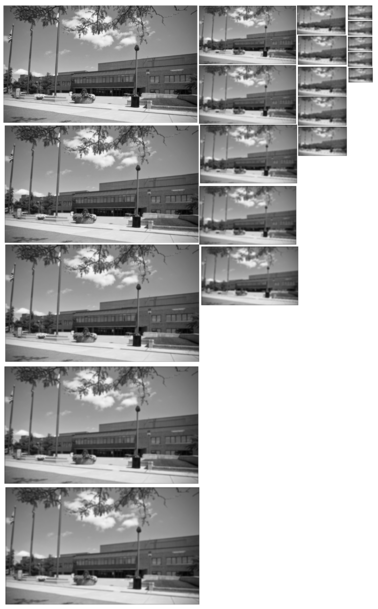
\includegraphics[scale=1.5]{./Gaussian_pyrmd.png}}
  			\caption{Gaussian Pyramid}
  		\label{gaussian-blurring}
\end{figure}
Each octave is half the previous one therefore function of "genOctave" generates octaves while genGaussianKernel function generates the kernels. The result obtained after blurring is seen in Fig{\ref{gaussian-blurring}} and {\ref{2nd-3rd-oct}} is what the question is asking. The resolution of second octave is 375 by 229 pixels while that of third octave is 118 by 114 pixels. 
\\
\begin{figure}
		\centering
  			\fbox{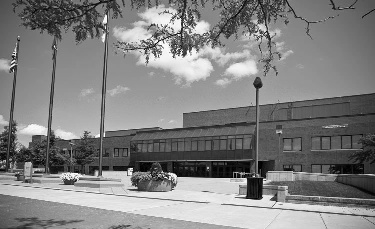
\includegraphics[scale=0.8]{./octave2_norm.jpg}
  			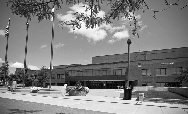
\includegraphics[scale=0.8]{./octave3_norm.jpg}}
  			\caption{Second and Third Octave}
  		\label{2nd-3rd-oct}
\end{figure}
The DoG images obtainted using the second and third octave are in fig:{\ref{2nd-3rd-dog}}
\begin{figure}
		\centering
  			\fbox{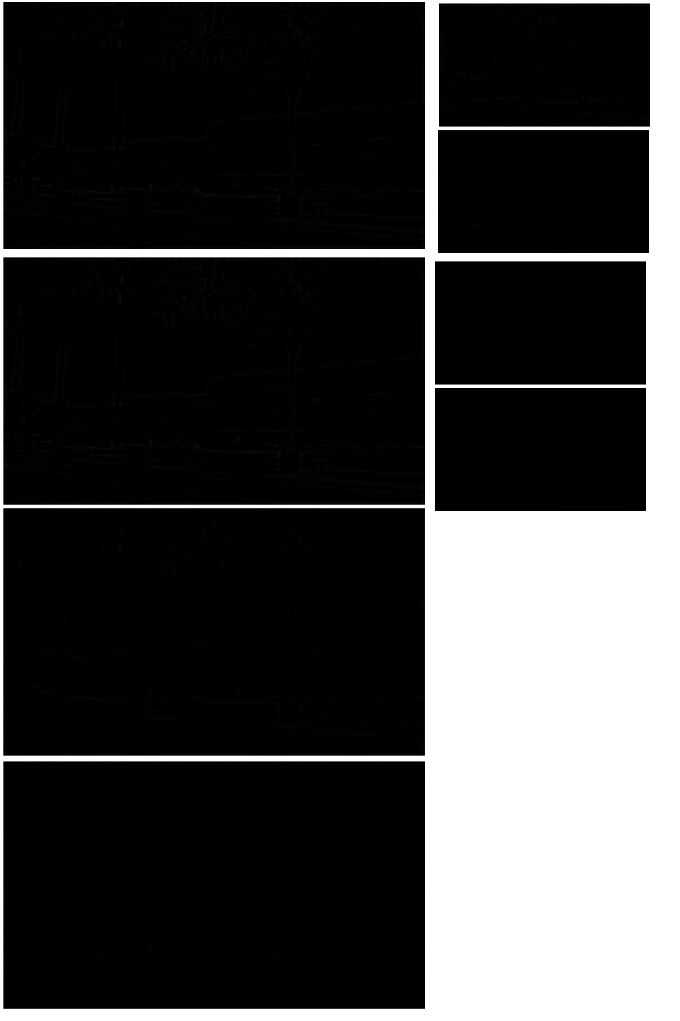
\includegraphics[scale=0.9]{./dog_pyrmd.png}}
  			\caption{Difference of Gaussians Pyramid}
  		\label{2nd-3rd-dog}
\end{figure}
\\
We perform first three steps of keypoint detection and plot the results back on the input image, see Fig{\ref{keypoint-result}}
\begin{figure}
		\centering
  			\fbox{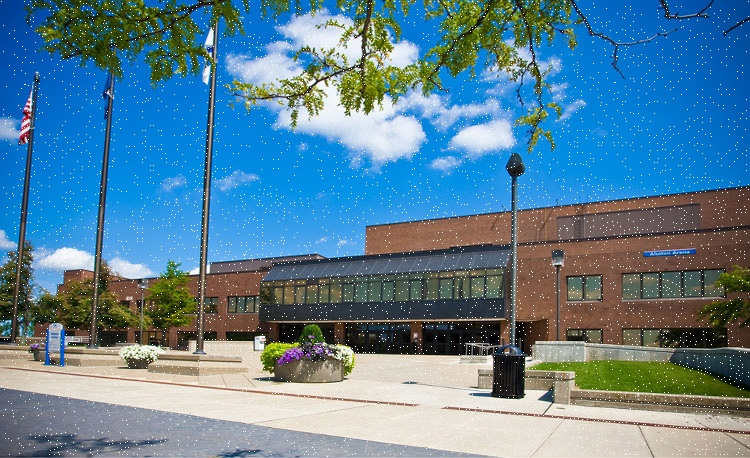
\includegraphics[scale=0.7]{./keypoints.jpg}}
  			\caption{Detected Keypoints on Original Image}
  		\label{keypoint-result}
\end{figure}
I think there are too many keypoints detected which are not relevant, I can see that in the top right corner, the keypoints are arranged perfectly on the branch, However, during areas of flat regions such as sky where everypoint is either a minima or a maxima we are having problems. Also, we havn't found subpixel keypoints. After doing these steps we could get a better result.
\\
The coordinates of the five left-most detected keypoints are(Format is (Height,Width) or (y,x)):
\\
(1,1),(1,24),(25,3),(4,28),(1,30)
\\
\\
Footnote:
\\
\\
I tried detecting the keypoints as well as I could. But I think that my convolution function is not quite right. I know the concept of keypoints detection and convolution, however, I was unable to implement it properly.
\end{answered}
		\item For the task of cursor detection, which aims to locate the cursor in an image, two sets of images and cursor templates, named as ”Set A” and ”Set B”, will be provided to you. Set A is composed of a total number of 25 images and 1 cursor template. Set A is for task 1., i.e., the basic cursor detection which contributes to 5 points. Set B is composed of a total number of 30 images and 3 different cursor template. Set B is for task 2.,
\\
i.e., which contributes to 3 bonus points.
\\
1. Detect cursors in Set A. [5 points]
\\
2. Detect cursors in Set B, which is more challenging. [3 bonus points]
\\
\\
Note that we will randomly select and run the code you submitted on a set of 20 withheld images to test the
performance of your cursor detection programs.
\begin{answered}
Method:
\\
\\
In the start I have had tested my previous code of keypoint detection on this problem, however, I couldn't get good results. I also tried on pulling cv2.SIFT from github repository(SIFT in OpenCV 3 is contrib package due to patent rights). This process made me realize that Difference of Gaussians work better with template matching. Therefore, we need edges and template matching performs better with edges. This also made me understand the difference between Template matching and feature based methods. The main pecularity of features is that during feature based matching we have to match features which might be skewed. However, in this task, the cursor is free from transanslation invariance. Moreover, after looking at the dataset, it seems that we need scale invariance.
\\
For scale invariance we are going to use what the Professor discussed about image stacks and resizing. We have two options to either resize the image or resize the template. However, if we sample the image and resize it it could happen that we might lose information.
\\
After comparing the performance of Laplacian and Canny on the given template, I hypothize that the result of canny would be better when pointer is behind different range of background due to the cursor wraped in one pixel boundary;See Fig.{\ref{wow-canny-wow}}. However, Canny is an edge detector, for an object like pointer it fails to detect it in some cases. See Fig.{\ref{canny-problem}}
\\
Therefore, I am taking Gaussian based approach for cursor detection.
\\
1. Basic Cursor Detection
For basic Cursor Detection firstly I tried running it without any downscaling or upscaling of the template. There was a 20$\%$ accuracy on these methods. After using downscaling and upscaling of templates in my program, I was able to boost my accuracy and detect almost all the points in the the basic Cursors. The accuracy as on writing this reports stands on not detecting any of negative images 10/10 and detecting 78.57$\%$ of positive pointers, which is 11 out of 14. Only 3 pointers were not detected. See {\ref{wow-basic-wow} and \ref{why-basic-why} } I am using a threshold of 0.6 to detect the pointers.
\begin{figure}
		\centering
  			\fbox{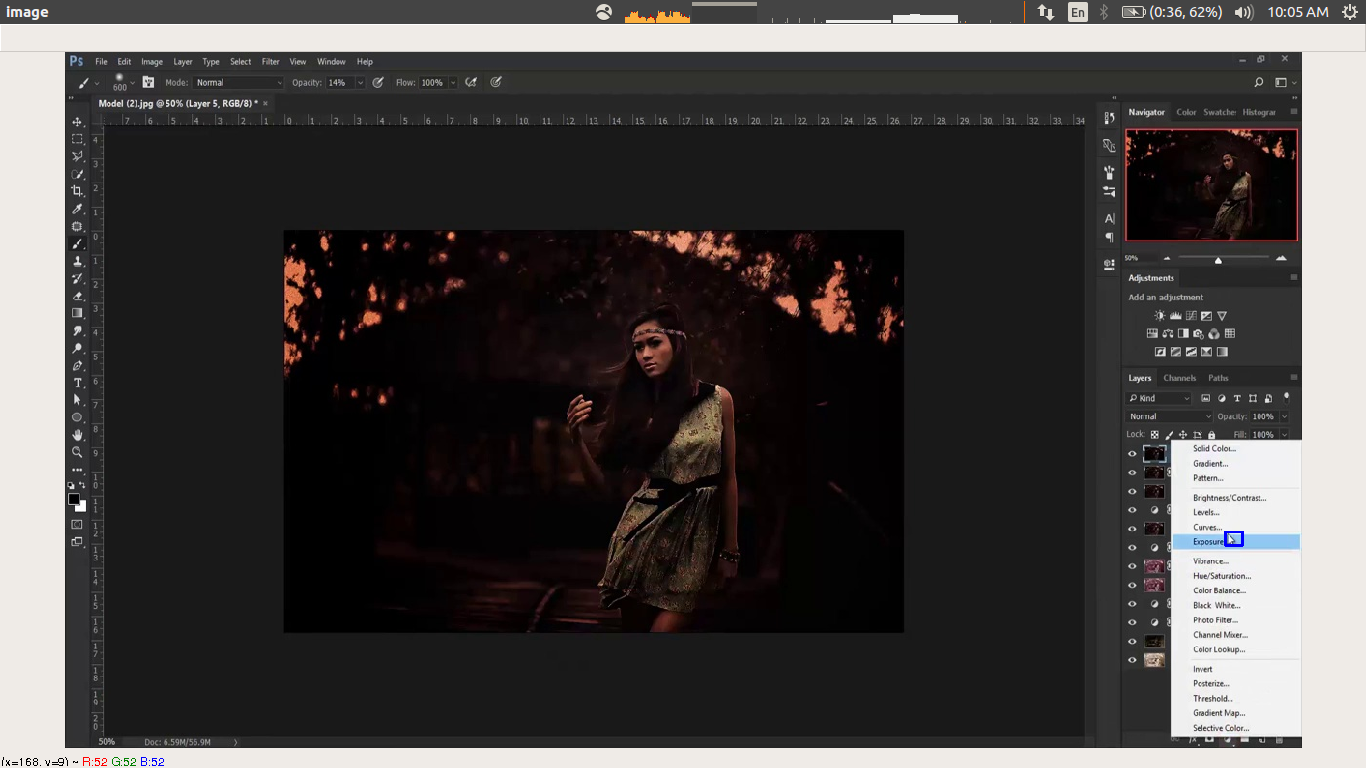
\includegraphics[scale=0.30]{./basic_cur_det.png}}
  			\caption{An example of good detection of cursor}
  		\label{wow-basic-wow}
\end{figure}
\begin{figure}
		\centering
  			\fbox{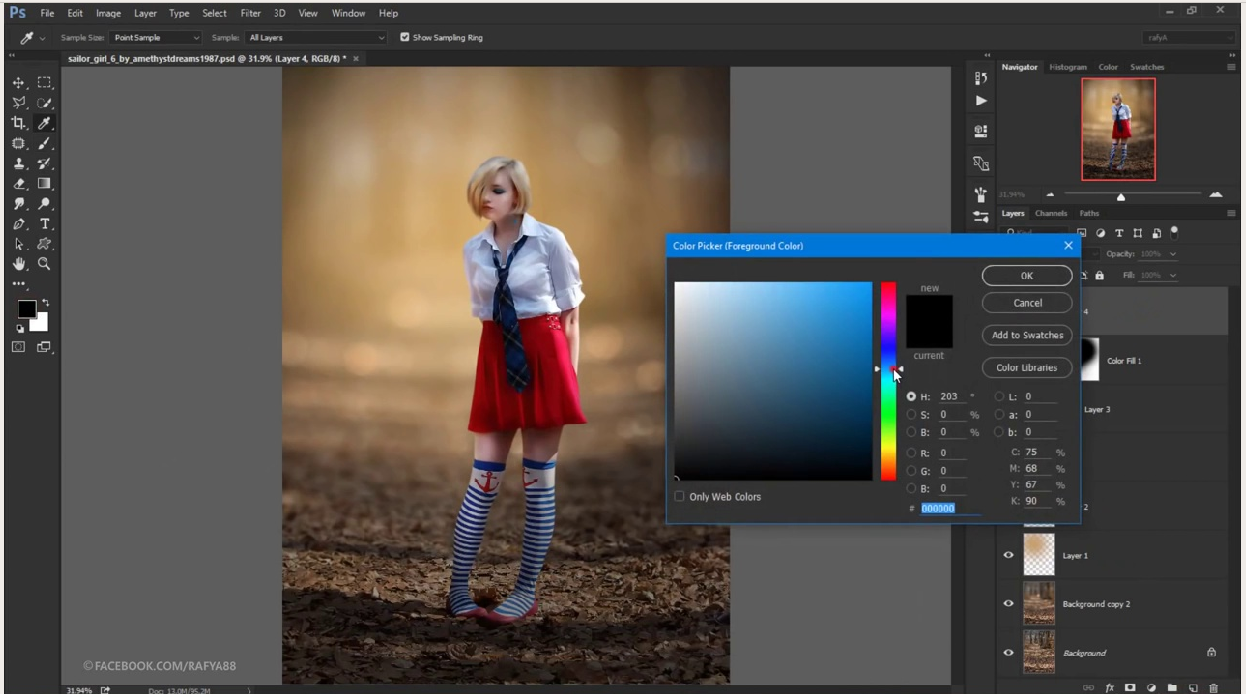
\includegraphics[scale=0.30]{./basic_cur_det_bad_case.png}}
  			\caption{Template Detection Failed to Detect any cursor}
  		\label{why-basic-why}
\end{figure}
\\
\\
2. Bonus Cursor Detection
\\
\\


\begin{figure}
		\centering
  			\fbox{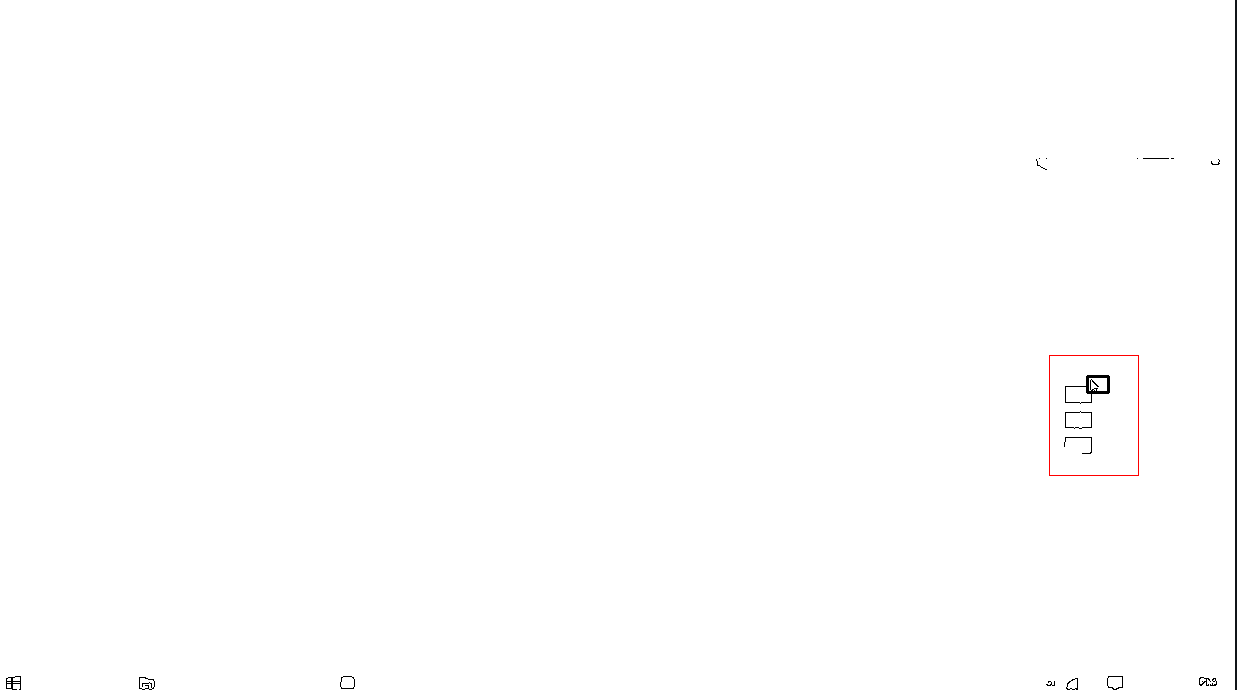
\includegraphics[scale=0.30]{./Cannyafter3scalings.png}}
  			\caption{pos$\_$3.jpg Using Canny after 3 downscalings (Inveted Image)}
  		\label{wow-canny-wow}
\end{figure}
\begin{figure}
		\centering
  			\fbox{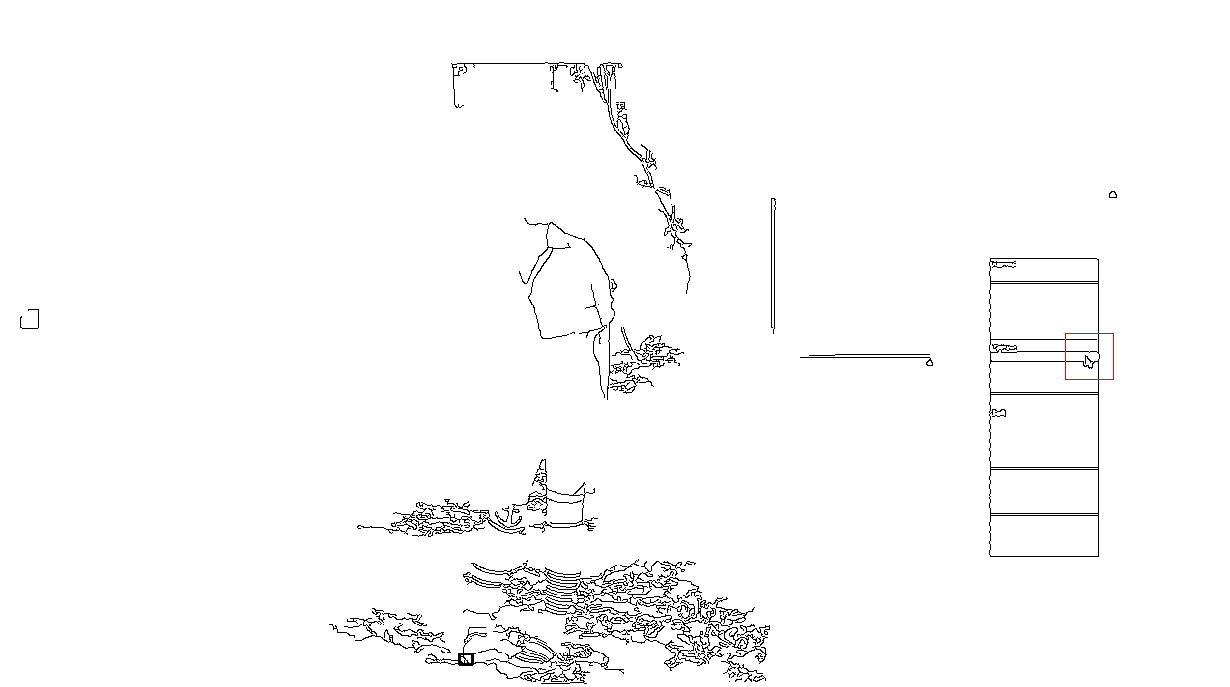
\includegraphics[scale=0.30]{./canyUnableToDetectcursor.png}}
  			\caption{pos$\_$9.jpg Red box shows that canny is unable to detect the cursor(Inveted Image)}
  		\label{canny-problem}
\end{figure}
\end{answered}
\end{QandA}
	\begin{thebibliography}{1}
							\bibitem{textbook} William Stallings, Lawrie Brown, Computer Security: Principles and Practice, 4th Edition
	\end{thebibliography}
\end{document}
